%From https://egu2018.eu/PICO_how-to_guide_to_PICO.pdf
%Abstracted and templated by Brian Ballsun-Stanton, Macquarie University.
%original template by https://github.com/snowtechblog/pico-latex-presentation by Anselm Köhler

\documentclass[unknownkeysallowed,usepdftitle=false, parskip=full]{beamer}
% unknownkeysallowed is needed for mac and the newer latex version -> is more picky than before...
\usetheme[headheight=1cm,footheight=2cm]{boxes}
%\usetheme{default}


\usepackage{default}
\usepackage{graphicx}

\usepackage{epsfig}
\usepackage{siunitx}
\usepackage{color}
\usepackage{ifthen}
%usepackage{ragged2e}

\usepackage[T1]{fontenc}
\usepackage[utf8]{inputenc}
%https://tex.stackexchange.com/a/203804/5483

\usepackage[activate={true,nocompatibility},final,tracking=true,kerning=true,spacing=true,factor=1100,stretch=10,shrink=10]{microtype} % http://www.khirevich.com/latex/microtype/
\microtypecontext{spacing=nonfrench}

\usepackage{lipsum} % for dummy text only
\usepackage[UKenglish]{babel} %https://tex.stackexchange.com/a/27743 
\usepackage[pangram]{blindtext} % https://tex.stackexchange.com/a/48411

%\usepackage{parskip} % from https://tex.stackexchange.com/q/11622
%\setlength{\parskip}{12pt} 

%\setparsizes{\parindent}{12pt}{\parfillskip}

%\usepackage{etoolbox} % as per https://tex.stackexchange.com/a/24331
%\appto\chapterheadendvskip{\vspace{-1\parskip}}
%\setparsizes{\parindent}{50pt plus 20pt minus 30pt}{\parfillskip}

\setbeamertemplate{navigation symbols}{}%remove navigation symbols
\setbeamersize{text margin left=1cm,text margin right=1cm}

% some colors
\definecolor{grau}{gray}{.5}
\definecolor{slfcolor}{rgb}{0.8313,0.5960,0.7058}
\definecolor{wslcolor}{rgb}{0.5686,0.1843,0.3686}

% setup links
\hypersetup{%
	%linkbordercolor=green,%
	colorlinks=false,%
	pdfborderstyle={/S/U/W 0},%
	%pdfpagemode=FullScreen,%
	pdfstartpage=4%
	}

% setup some fonts
\setbeamerfont{title}{series=\bfseries, size=\small}
\setbeamerfont{author}{size*={5pt}{0pt}}
\setbeamerfont{institute}{size*={3pt}{0pt}}
\setbeamerfont{bodytext}{size=\scriptsize}
	
% Title setup	
\title{FOAR705 Pico Presentation}
\author{Matthew Clark (\texttt{matthew.clark3@hdr.mq.edu.au})}
\institute{Macquarie University, Sydney, NSW}
% add title in headbox
\setbeamertemplate{headline}
{\leavevmode
\begin{beamercolorbox}[width=1\paperwidth]{head title}
  % LOGO
  \begin{columns}[t, totalwidth=\textwidth]
  \begin{column}[c]{1.05cm}
     
\includegraphics[width=1cm]{figure/logo1.jpg}
  \end{column}
  % TITLE
   \begin{column}[c]{10.6cm}
   \centering \usebeamerfont{title} \textcolor{slfcolor}{\inserttitle} \\
   \centering \usebeamerfont{author} \color[rgb]{0,0,0} \insertauthor \\
   \vspace{-0.05cm}
   \centering \usebeamerfont{institute} \insertinstitute
  \end{column}
  % PICTURE
  \begin{column}[c]{1.15cm}
    \hspace{0.005cm}
    
\includegraphics[width=1cm]{figure/logo1.jpg}
  \end{column}
  \end{columns}
  {\color{slfcolor}\hrule height 1pt\vspace{0.1cm}}
\end{beamercolorbox}%
}

% setup the navigation in footbox
% first set some button colors
\newcommand{\buttonactive}{\setbeamercolor{button}{bg=wslcolor,fg=white}}
\newcommand{\buttonpassive}{\setbeamercolor{button}{bg=slfcolor,fg=black}}
% now set up that the one active one gets the new color.
\newcommand{\secvariable}{nothing}
% therefore we write before each section (well, everything which should be part of the navi bar)
% the variable \secvariable to any name which is in the next function ...
\newcommand{\mysection}[1]{\renewcommand{\secvariable}{#1}
}
% ... compaired to strings in the following navibar definition ...
\newcommand{\tocbuttoncolor}[1]{%
 \ifthenelse{\equal{\secvariable}{#1}}{%
    \buttonactive}{%
    \buttonpassive}
 }
% ... here we start to set up the navibar. each entry is calling first the function \tocbuttoncolor with the argument which should be tested for beeing active. if active, then change color. afterwards the button is draw. so to change that, you need to change the argument in \toc..color, the first in \hyperlink and before each frames definition... A bit messed up, but works...
\newlength{\buttonspacingfootline}
\setlength{\buttonspacingfootline}{-0.2cm}
\setbeamertemplate{footline}
{\leavevmode
\begin{beamercolorbox}[width=1\paperwidth]{head title}
  {\color{slfcolor}\hrule height 1pt}
  \vspace{0.05cm}
  % set up the buttons in an mbox
  \centering \mbox{
    \tocbuttoncolor{2minutemadness}
    \hyperlink{2minutemadness}{\beamerbutton{2 Minute Madness}}
    \tocbuttoncolor{background}
    \hspace{\buttonspacingfootline}
      \hyperlink{background}{\beamerbutton{Background}}
    \tocbuttoncolor{Intention}
    \hspace{\buttonspacingfootline}
      \hyperlink{Intention}{\beamerbutton{Intention}}
    \tocbuttoncolor{Execution}
    \hspace{\buttonspacingfootline}
      \hyperlink{Execution}{\beamerbutton{Execution}}
    \tocbuttoncolor{limitations}
    \hspace{\buttonspacingfootline}
      \hyperlink{Limitations}{\beamerbutton{Limitations}}
    \tocbuttoncolor{Results}
    \hspace{\buttonspacingfootline}
      \hyperlink{Results}{\beamerbutton{Results}}
    \tocbuttoncolor{conclusion}
    \hspace{\buttonspacingfootline}
      \hyperlink{conclusion}{\beamerbutton{Conclusion}}
    % this last one should normaly not be used... it will open the preferences to change the 
    % behaviour of the acrobat reader in fullscreen -> usefull in pico...
    \setbeamercolor{button}{bg=white,fg=black}
    % for presentation
    %\hspace{-0.1cm}\Acrobatmenu{FullScreenPrefs}{\beamerbutton{\#}}
    % for upload
    
     
\Acrobatmenu{FullScreenPrefs}{\vspace{0.3cm}\hspace{0.24cm}\mbox{%
      
\includegraphics[height=0.04\textheight,keepaspectratio]{%
	  figure/CreativeCommons_Attribution_License.eps}%
	  }}
   }
    \vspace{0.05cm}
\end{beamercolorbox}%
}


\begin{document}


%%%%%%%%%%%%%%%%%%%%%%%%%%%%%%%%%%%%%%%%%%%%%%%%%%%%%%%%%%%%%%%%%%%%%%%%%%
\mysection{2minutemadness}
%%%%%%%%%%%%%%%%%%%%%%%%%%%%%%%%%%%%%%%%%%%%%%%%%%%%%%%%%%%%%%%%%%%%%%%%%%
\begin{frame}\label{\secvariable}
\begin{center}
    \textbf{Background and Implementation}
    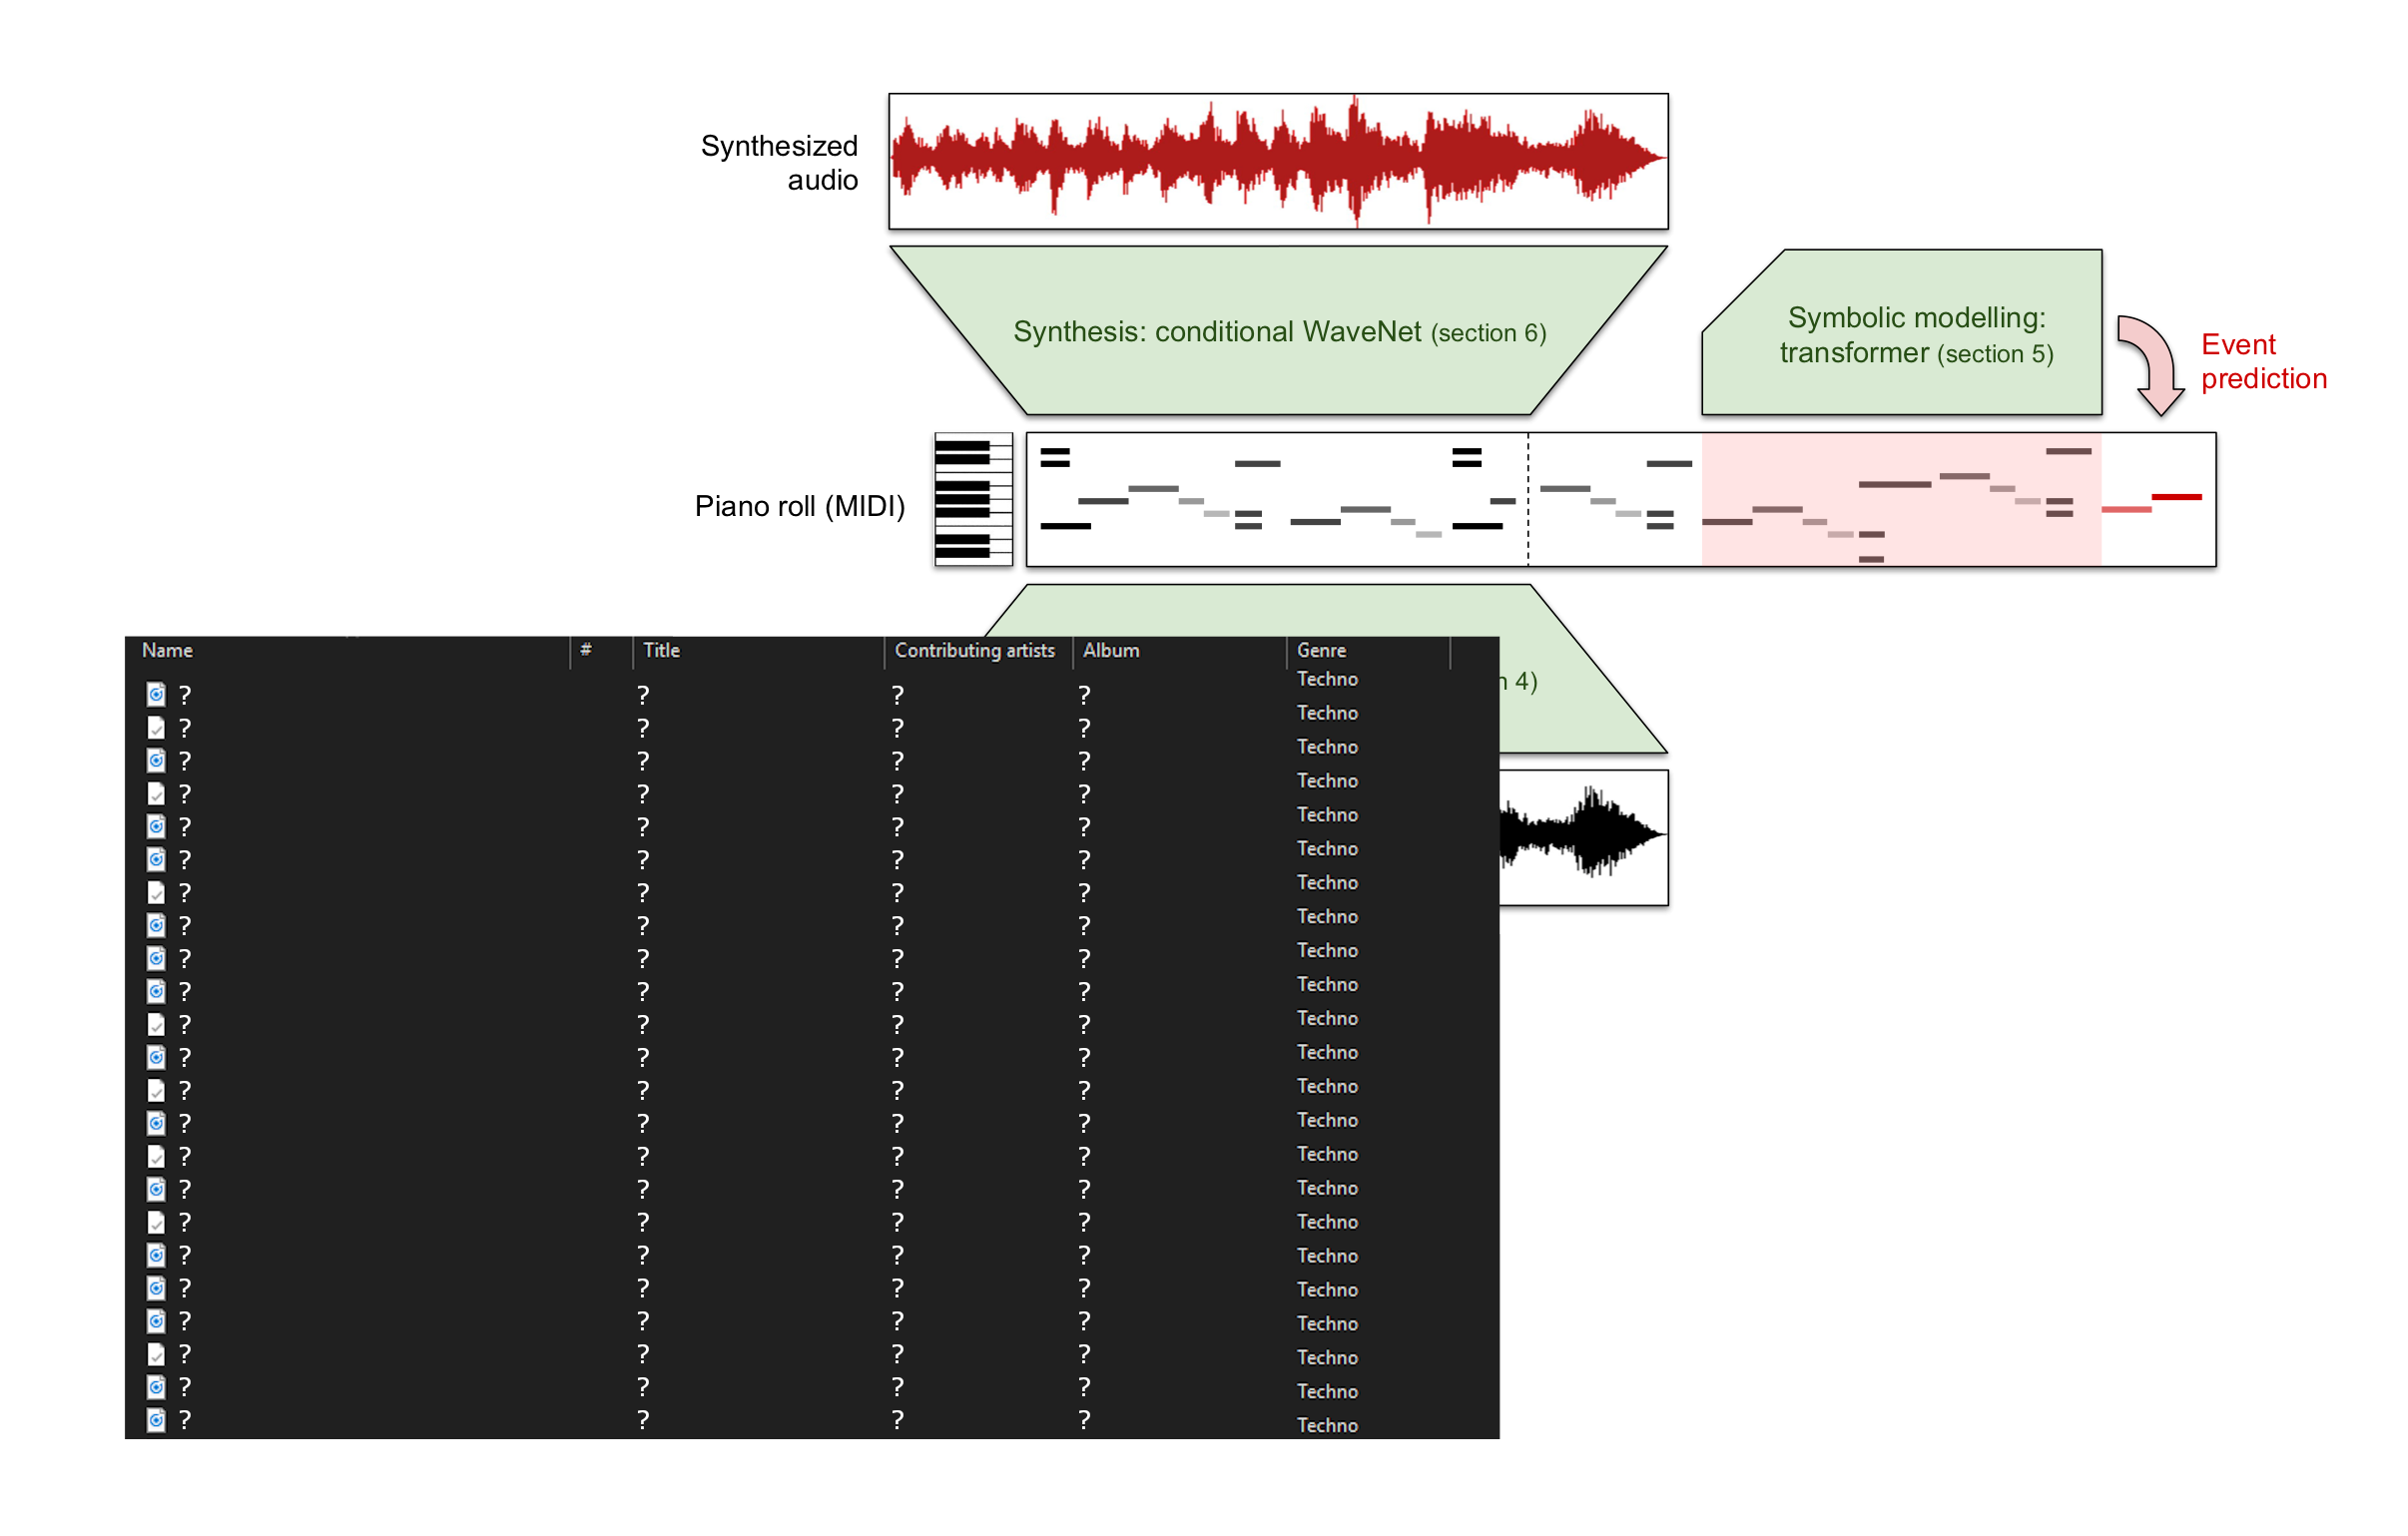
\includegraphics[width=1\textwidth,height=1\textheight,keepaspectratio]{%
figure/slide1.png}
\end{center}
\end{frame}

\begin{frame}\label{\secvariable}
\begin{center}
\textbf{Execution and Relevance}
    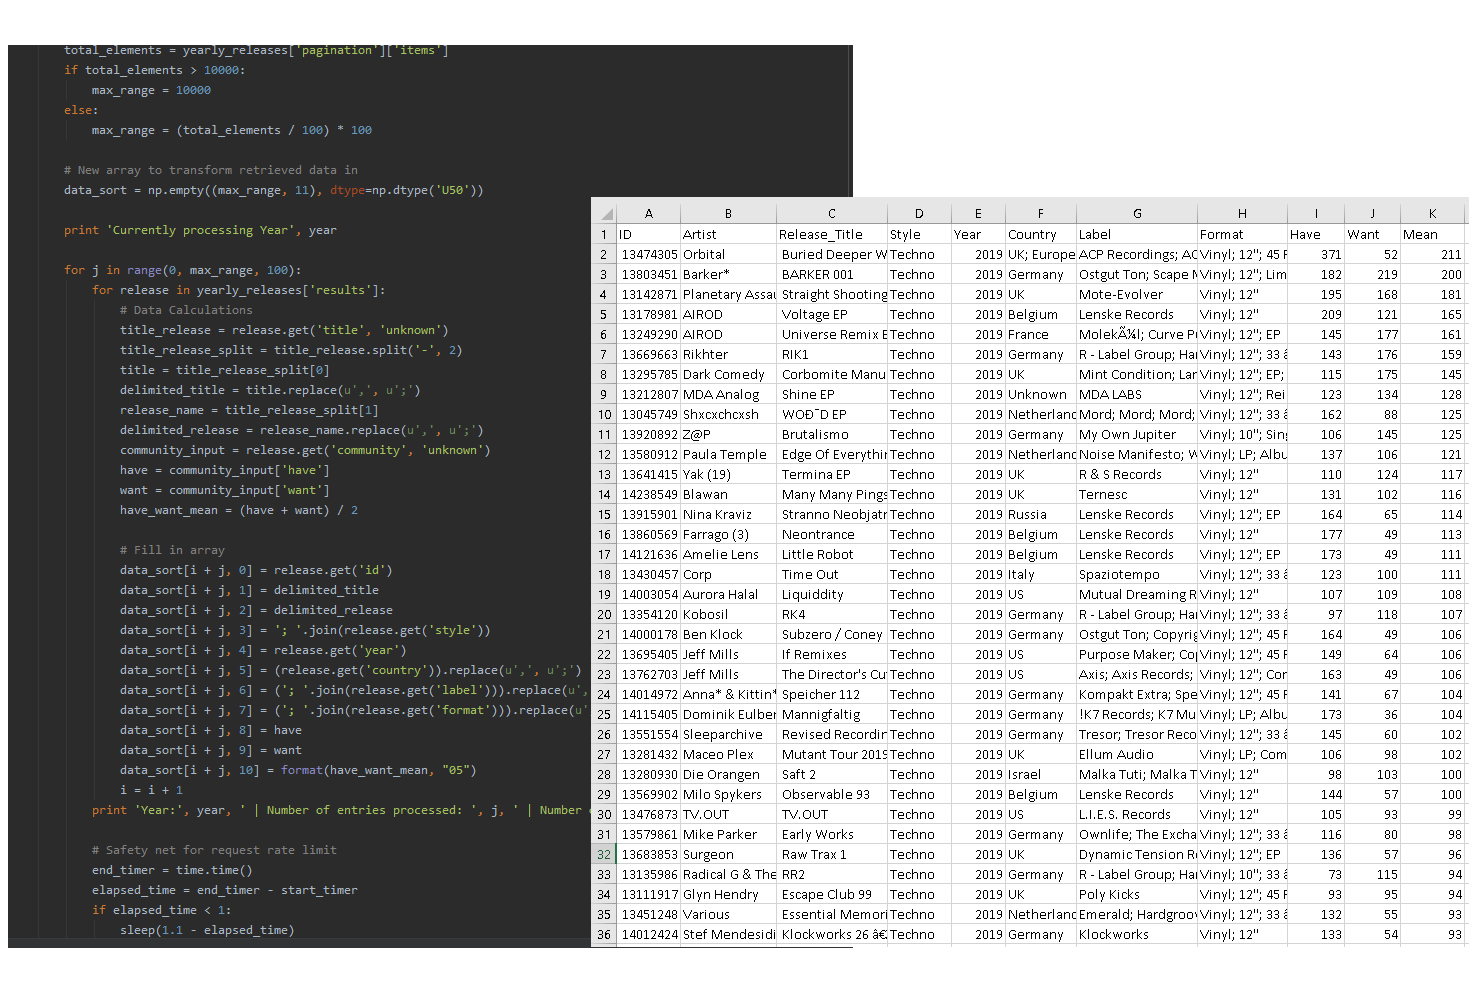
\includegraphics[width=1\textwidth,height=1\textheight,keepaspectratio]{%
figure/slide2.png}
\end{center}
\end{frame}

%%%%%%%%%%%%%%%%%%%%%%%%%%%%%%%%%%%%%%%%%%%%%%%%%%%%%%%%%%%%%%%%%%%%%%%%%%
\mysection{background}
%%%%%%%%%%%%%%%%%%%%%%%%%%%%%%%%%%%%%%%%%%%%%%%%%%%%%%%%%%%%%%%%%%%%%%%%%%
\begin{frame}\label{\secvariable}
  \begin{columns}[t]
  %https://tex.stackexchange.com/a/7452/5483
    \begin{column}[c]{0.60\textwidth}
    \parbox{\linewidth}{
    My thesis will be looking into the development of a techno data set that can be used for the purposes of machine learning to produce a creative artificial intelligence program. As there is currently no techno-based data set available, I will need to construct one.\\
	However before I create the data set, I need to identify what songs I want to use for the data set. Because techno music has evolved over the past 30 years, I want a data set which encompasses the most popular techno songs streching over those 30 years.
      }
    \end{column}
    \begin{column}[c]{0.30\textwidth}
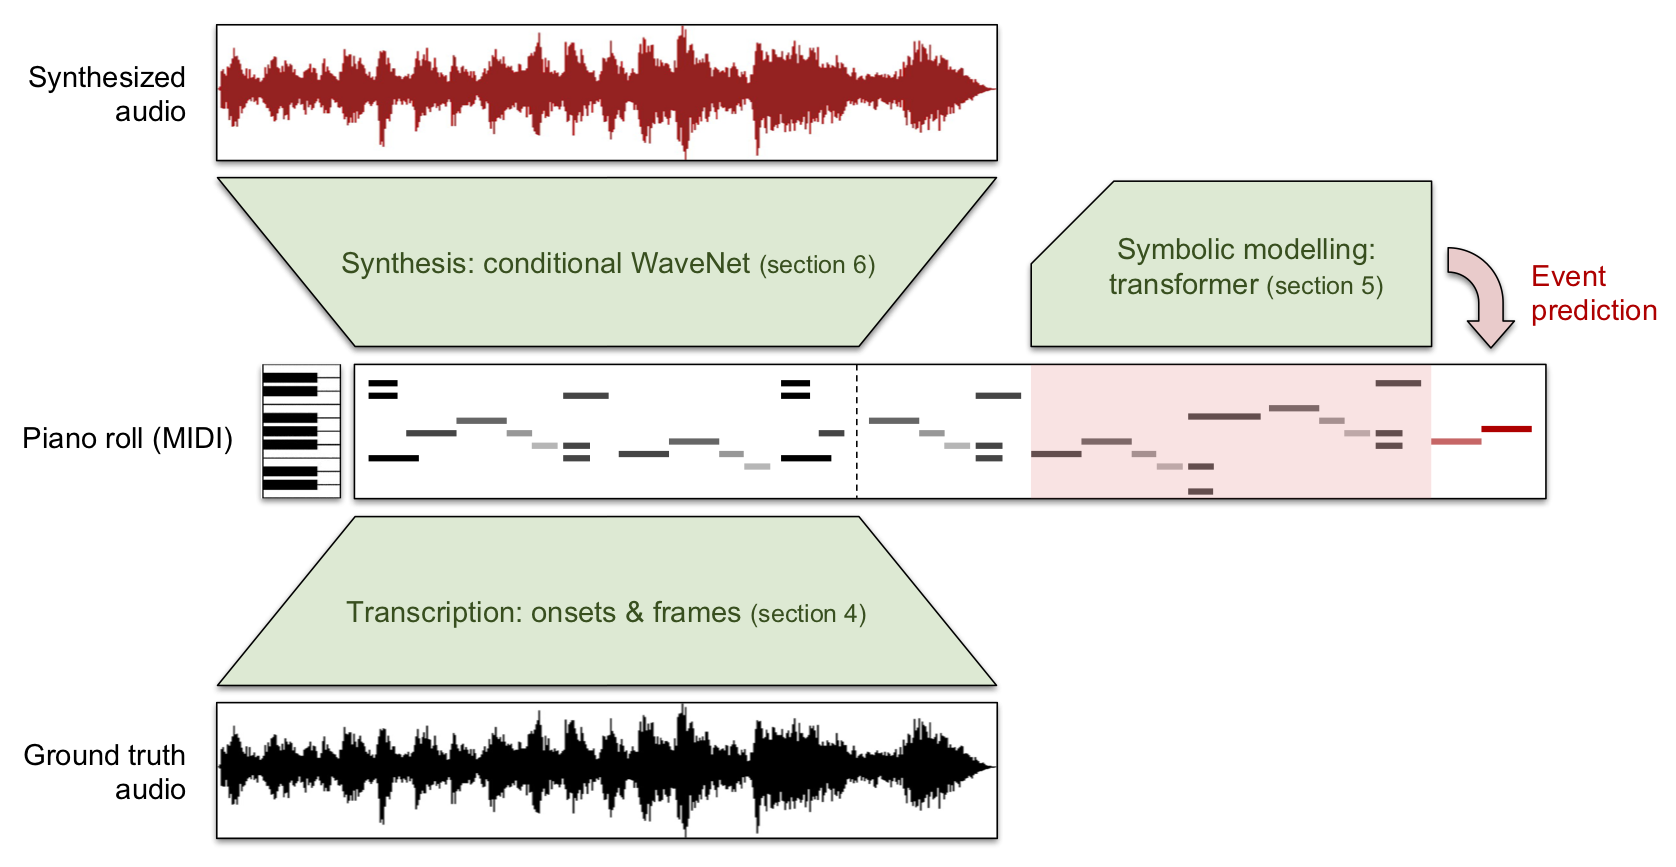
\includegraphics[width=1\textwidth,height=0.5\textheight,keepaspectratio]{%
figure/mididata.png}\\
\vspace{12pt}
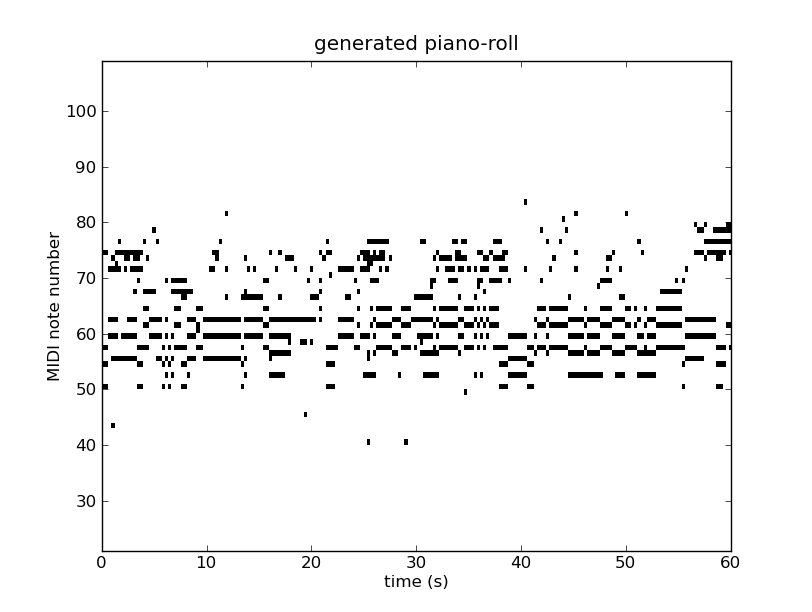
\includegraphics[width=1\textwidth,height=0.5\textheight,keepaspectratio]{%
figure/slide3_1.png}
    \end{column}
  \end{columns}
\end{frame}

%%%%%%%%%%%%%%%%%%%%%%%%%%%%%%%%%%%%%%%%%%%%%%%%%%%%%%%%%%%%%%%%%%%%%%%%%%
\mysection{Intention}
%%%%%%%%%%%%%%%%%%%%%%%%%%%%%%%%%%%%%%%%%%%%%%%%%%%%%%%%%%%%%%%%%%%%%%%%%%
\begin{frame}\label{\secvariable}
  \begin{columns}[t]
  %https://tex.stackexchange.com/a/7452/5483
    \begin{column}[c]{0.30\textwidth}
%slide4_1: https://www.billboard.com/articles/business/digital-and-mobile/8526654/discogs-nearmint-professional-record-sellers
%slide4_2: https://www.sparefoot.com/self-storage/blog/20388-how-to-move-your-vinyl-record-collection-cross-country/

\includegraphics[width=1\textwidth,height=0.5\textheight,keepaspectratio]{%
figure/slide4_1.jpg}\\
\vspace{12pt}
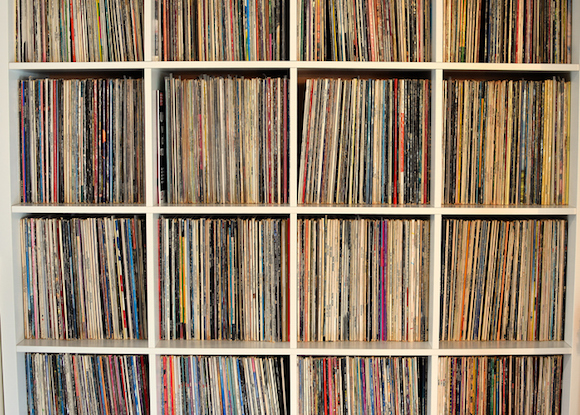
\includegraphics[width=1\textwidth,height=0.5\textheight,keepaspectratio]{%
figure/slide4_2.jpg}
    \end{column}
    \begin{column}[c]{0.60\textwidth}
    \parbox{\linewidth}{
    The intention of this proof of concept is to be able to use Discog's API to extract the top 100 techno songs based on the mean of an entries 'have' and 'want' values for every year between 1989 - 2019, before exporting to a csv; 'have' referring to the number of uses who state they own the release compared to those who 'want' the release.\\
    The script is intended to clean the data set before exporting, including removing duplicates, fixing nulls, and parsing unwanted commas.
     }
    \end{column}
  \end{columns}
\end{frame}

%%%%%%%%%%%%%%%%%%%%%%%%%%%%%%%%%%%%%%%%%%%%%%%%%%%%%%%%%%%%%%%%%%%%%%%%%%
\mysection{Execution}
%%%%%%%%%%%%%%%%%%%%%%%%%%%%%%%%%%%%%%%%%%%%%%%%%%%%%%%%%%%%%%%%%%%%%%%%%%
\begin{frame}\label{\secvariable}
  \begin{columns}[t]
  %https://tex.stackexchange.com/a/7452/5483
    \begin{column}[c]{0.70\textwidth}
    \parbox{\linewidth}{
    The developed python script executes the following:
    \begin{enumerate}
        \item Authenticates with the API
        \item Creates a dataset array with relevant headings
        \item Starts a for loop from 2019 to 1989
        \item Extracts the top 10000 entries by relevance and places them into an array
        \item Removes entries which contain more than 1 style
        \item Removes duplicates
        \item Sorts by mean and concatenates the top 100 entries to a dataset array
    \end{enumerate}
    Once this has completed, the dataset array is exported as a csv file
      }
    \end{column}
    \begin{column}[c]{0.35\textwidth}
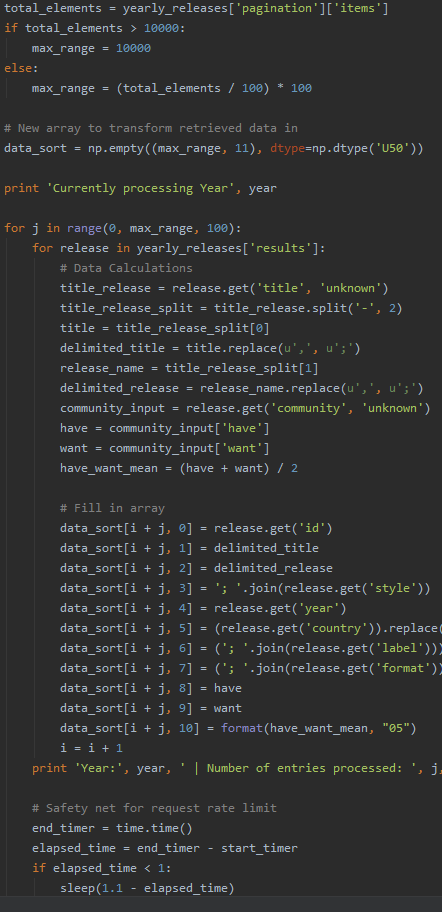
\includegraphics[width=1\textwidth,height=1\textheight,keepaspectratio]{%
figure/slide5.png}\\
    \end{column}
  \end{columns}
\end{frame}

%%%%%%%%%%%%%%%%%%%%%%%%%%%%%%%%%%%%%%%%%%%%%%%%%%%%%%%%%%%%%%%%%%%%%%%%%%
\mysection{Limitations}
%%%%%%%%%%%%%%%%%%%%%%%%%%%%%%%%%%%%%%%%%%%%%%%%%%%%%%%%%%%%%%%%%%%%%%%%%%
\begin{frame}\label{\secvariable}
\parbox{\linewidth}{
\textbf{Discogs' API's Limitations:}
\begin{itemize}
    \item Discogs catalogs releases, not individual tracks
    \item Discogs will only retrieve a maximum of 10,000 entries per search request
    \item Each individual request can only retrieve a page of 100 entries
    \item There is a rate limit of 60 requests per minute, resulting in a 50 minute run time with a timer running as a safeguard
    \item Discogs will produce numerous duplication of entries, which are removed prior to sorting
    \item When retrieving 'Techno' releases, it will include multi-style releases which contain 'techno as one of their styles - these are removed before added to the dataset
\end{itemize}
}
\end{frame}




%%%%%%%%%%%%%%%%%%%%%%%%%%%%%%%%%%%%%%%%%%%%%%%%%%%%%%%%%%%%%%%%%%%%%%%%%%
\mysection{Results}
%%%%%%%%%%%%%%%%%%%%%%%%%%%%%%%%%%%%%%%%%%%%%%%%%%%%%%%%%%%%%%%%%%%%%%%%%%
\begin{frame}\label{\secvariable}
\begin{center}
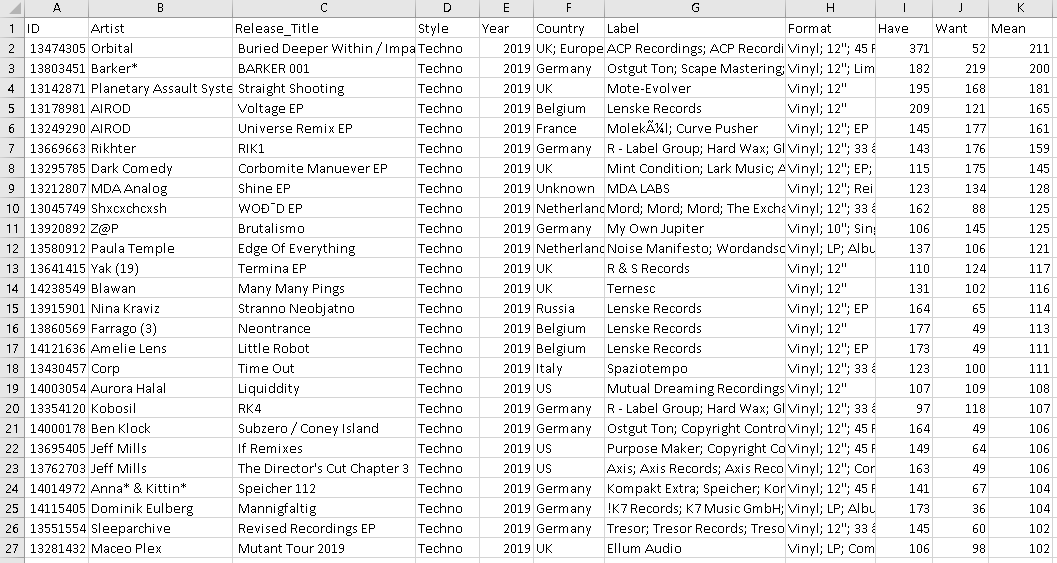
\includegraphics[width=1\textwidth,height=0.7\textheight,keepaspectratio]{%
figure/slide8.png}
\end{center}
\vspace{-0.2cm}

The results are cleaned as the program runs, and automatically exports the data set to a csv file. The resulting file has a column for the headings following by 3000 entries sorted by its mean value and by year.

\end{frame}


%%%%%%%%%%%%%%%%%%%%%%%%%%%%%%%%%%%%%%%%%%%%%%%%%%%%%%%%%%%%%%%%%%%%%%%%%%
\mysection{conclusion}
%%%%%%%%%%%%%%%%%%%%%%%%%%%%%%%%%%%%%%%%%%%%%%%%%%%%%%%%%%%%%%%%%%%%%%%%%%
\begin{frame}\label{\secvariable}
\textbf{In Summary:}
\begin{itemize}
    \item This proof of concept produces a data set of meta data containing the top 100 techno releases from 1989 - 2019
    \item The relevance of this is it can be used to quantitatively choose the contents of a data set when developing a set for the purposes of machine learning
    \item The proof of concept is implemented in python using Discogs' API
    \item The script extracts and transforms data year by year, cleaning as it goes. The top 100 tracks are sliced from the rest of the sorted set and concatenated to the dataset array
    \item After execution, the dataset array is exported to a csv file
    \item The average run time is roughly 50 minutes due to the API's request limit.
\end{itemize}
  
\end{frame}



\end{document}
